%! Author = antoniomasotti
%! Date = 25.11.23

\subsection{Definitions}
\begin{frame}{Contracts}
    \begin{block}{Contracts}
        \textit{A formal agreement between parties or individual.
        Synonyms: pact, agreement, protocol, deal}

        --- Oxford English Dictionary
    \end{block}

    \begin{block}{Contract Testing}
        \textit{A contract test is a test at the boundary of an external service, verifying
        that it meets the contract expected by a consuming service.}

        --- Martin Fowler
    \end{block}

\end{frame}

\subsection{Understanding contracts}
\begin{frame}{A pact between who?}

    \only<1-2>{
    \begin{itemize}
        \item \textbf{Consumer}: the service that consumes the information (typically closer to the user)
        \item \textbf{Provider}: the service that provides the information (typically closer to the data)
    \end{itemize}
    }

    \only<2>{
    \vspace{.5cm}
    \textbf{Where do we find this architecture?}

    \begin{itemize}
        \item REST, GraphQL, gRPC, SOAP \ldots APIs
        \item Microservices communication (over TCP, HTTP, Quic, AMQP, \ldots)
        \item SOA
        \item Other kinds of distributed systems (IoT, \ldots)
        \item Client-Server
        \item Messaging systems (Kafka, RabbitMQ, SQS \ldots)
        \item Notifying systems (Webhooks, SNS, \ldots)
    \end{itemize}
    }
\end{frame}

\begin{frame}{The role of contracts in testing}
    \begin{center}
        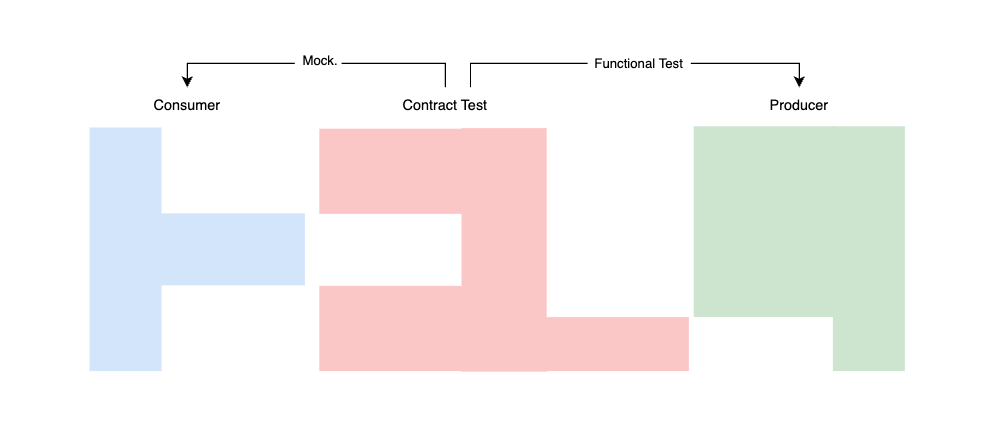
\includegraphics[scale=.3]{./assets/contract_divided}
        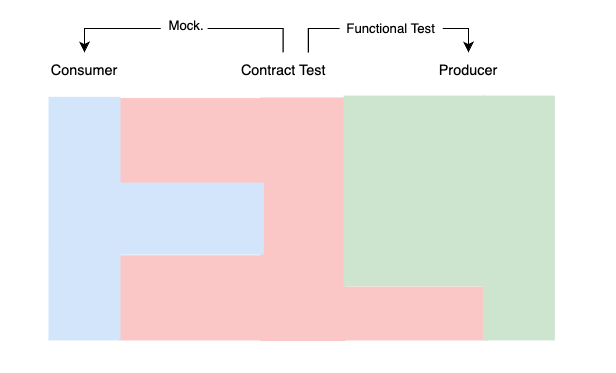
\includegraphics[scale=.3]{./assets/contract_united}
    \end{center}
\end{frame}

\begin{frame}{Who does initiate the contract?}
    Both parties can initiate the contract, \textbf{but...}

    Here I will present you the \textbf{Consumer Driven Contracts} approach.
\end{frame}

\begin{frame}{Provider driven contracts}
    \only<1>{
    \begin{center}
        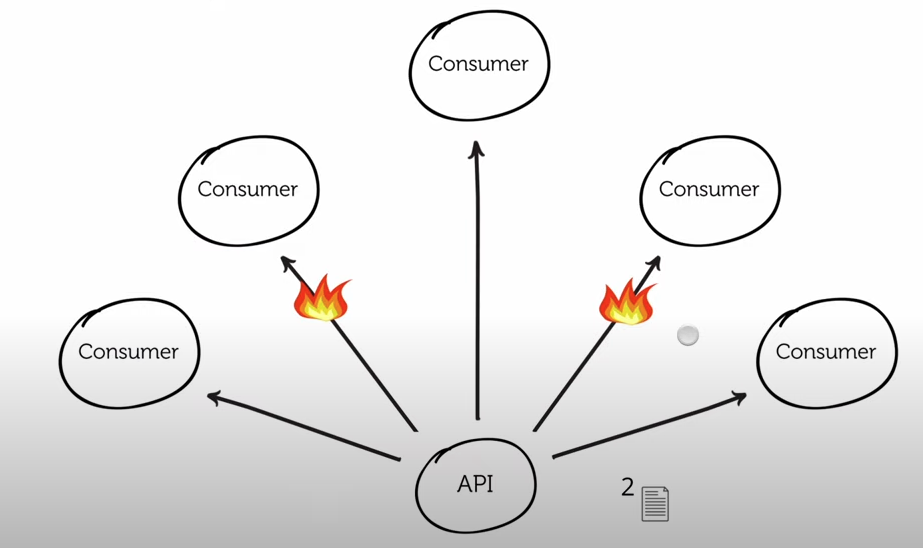
\includegraphics[scale=.3]{./assets/provider_driven}
    \end{center}
    }

    \only<2>{
    \begin{center}
        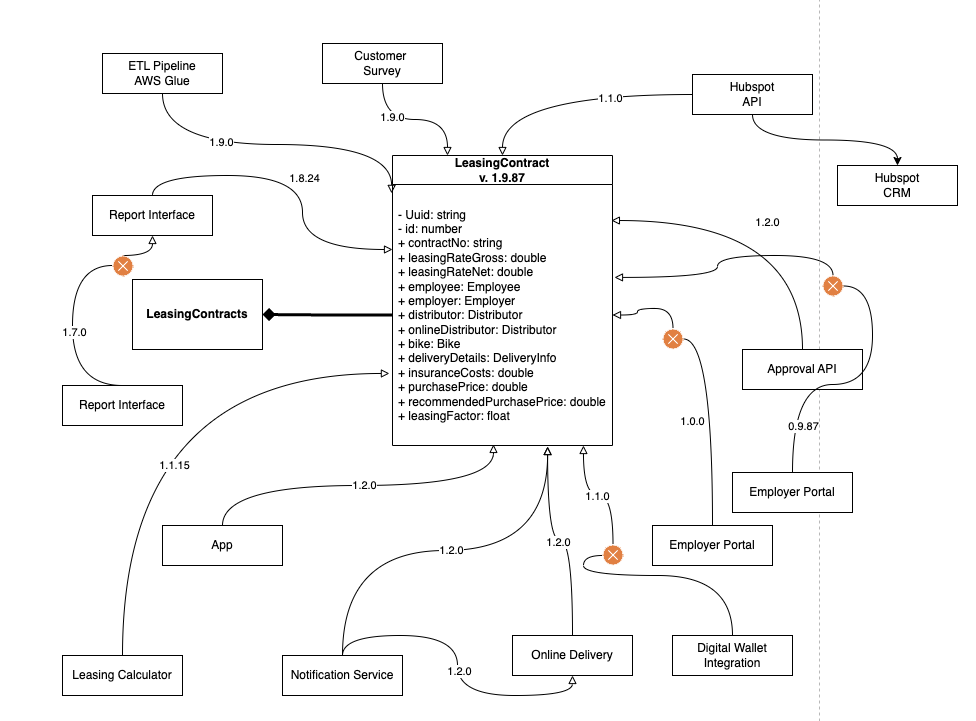
\includegraphics[scale=.3]{./assets/model3}
    \end{center}
    }


\end{frame}

\begin{frame}{Consumer Driven Contracts}
    \begin{shadequote}
        \hspace{.5cm}
        A strange inversion of reasoning\ldots -- D. Dennet
    \end{shadequote}
    \textit{}

    \only<1>{
    \begin{center}
        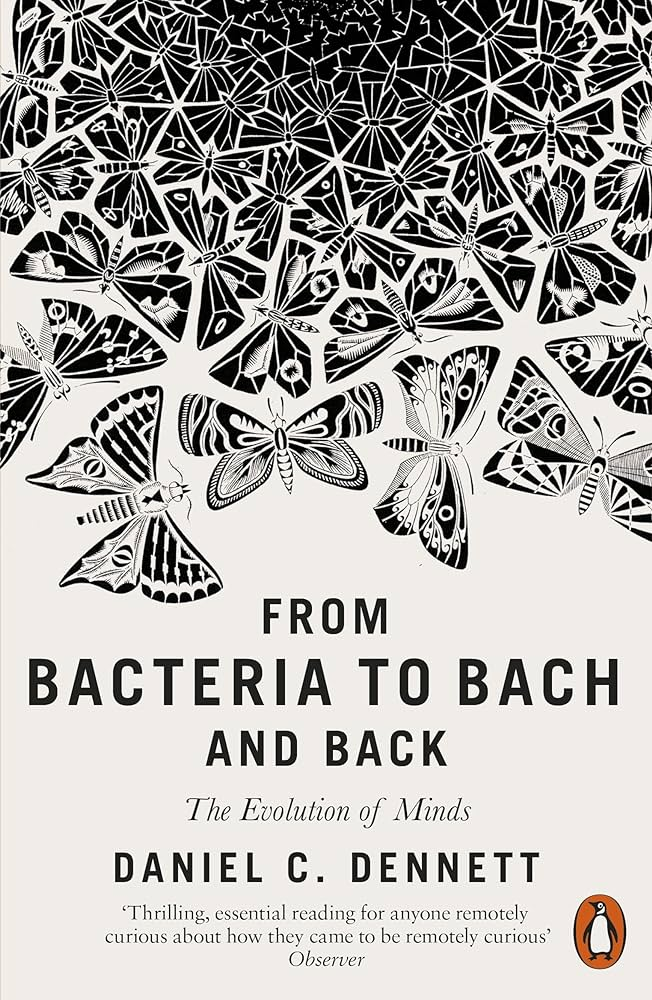
\includegraphics[height=.6\textheight]{./assets/bacteria}
        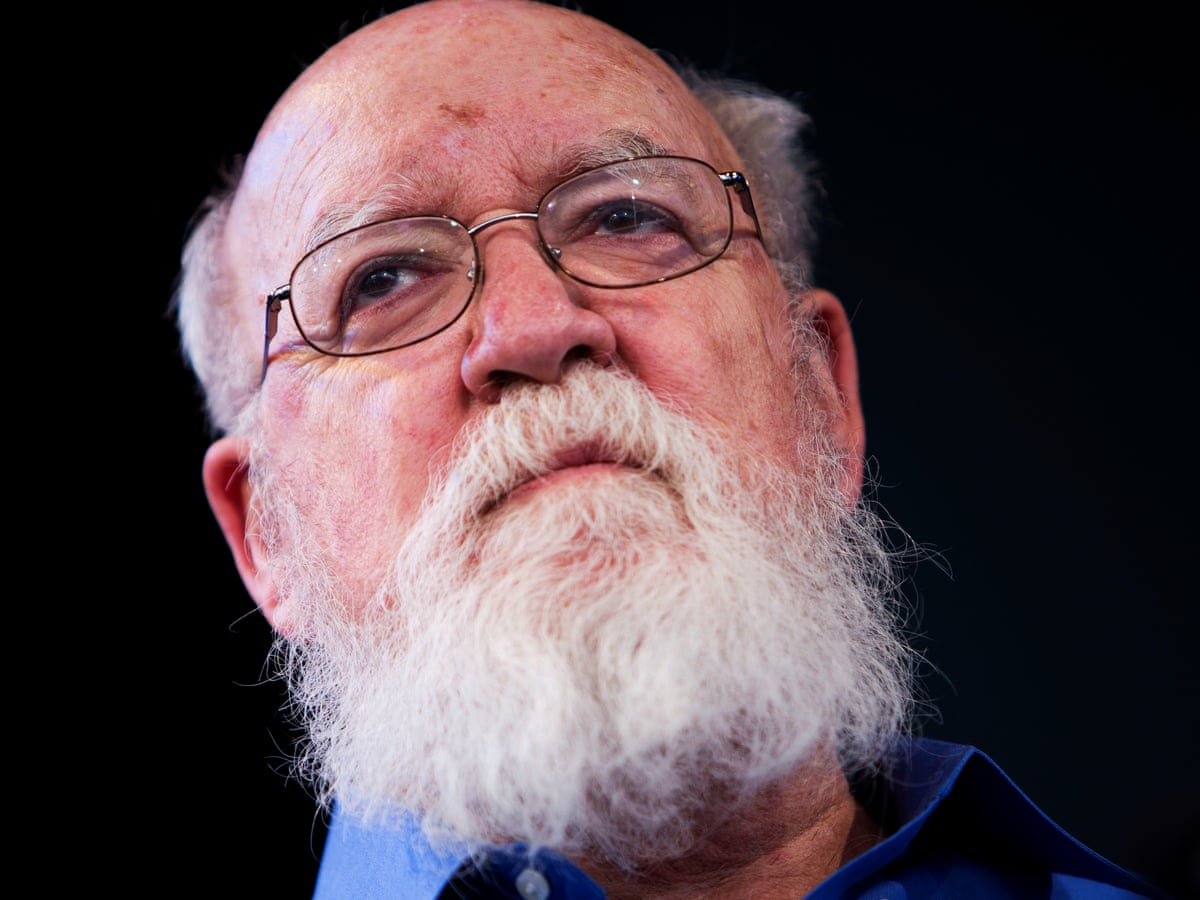
\includegraphics[height=.4\textheight]{./assets/dennet}
    \end{center}
    }

    \only<2>{
    \begin{center}
        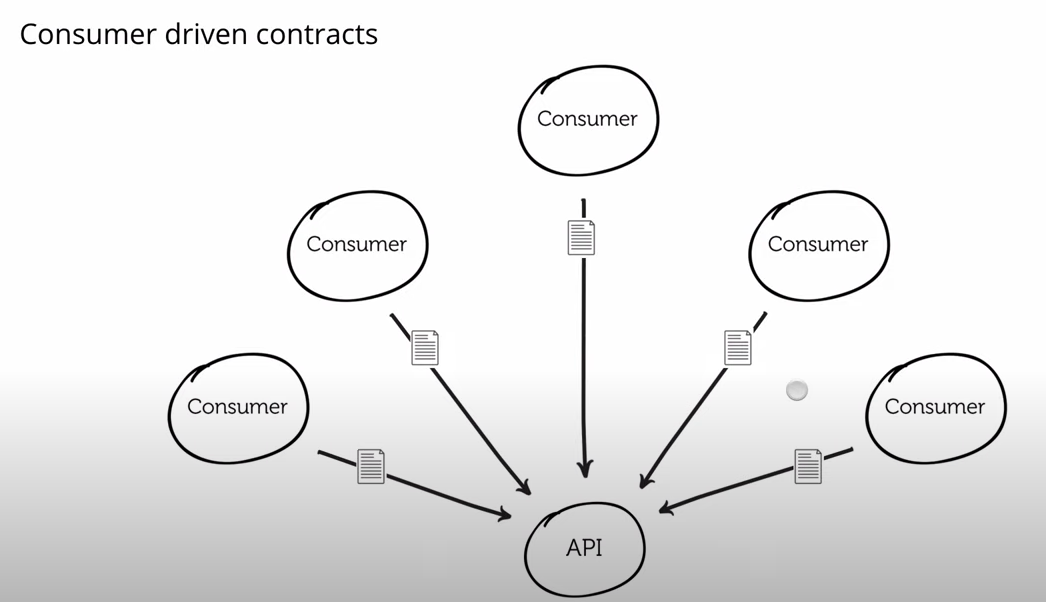
\includegraphics[width=.8\textwidth]{./assets/consumer_driven}
    \end{center}
    }
\end{frame}


\subsection{Pact}
\begin{frame}{Pact - Overview}
    \begin{center}
        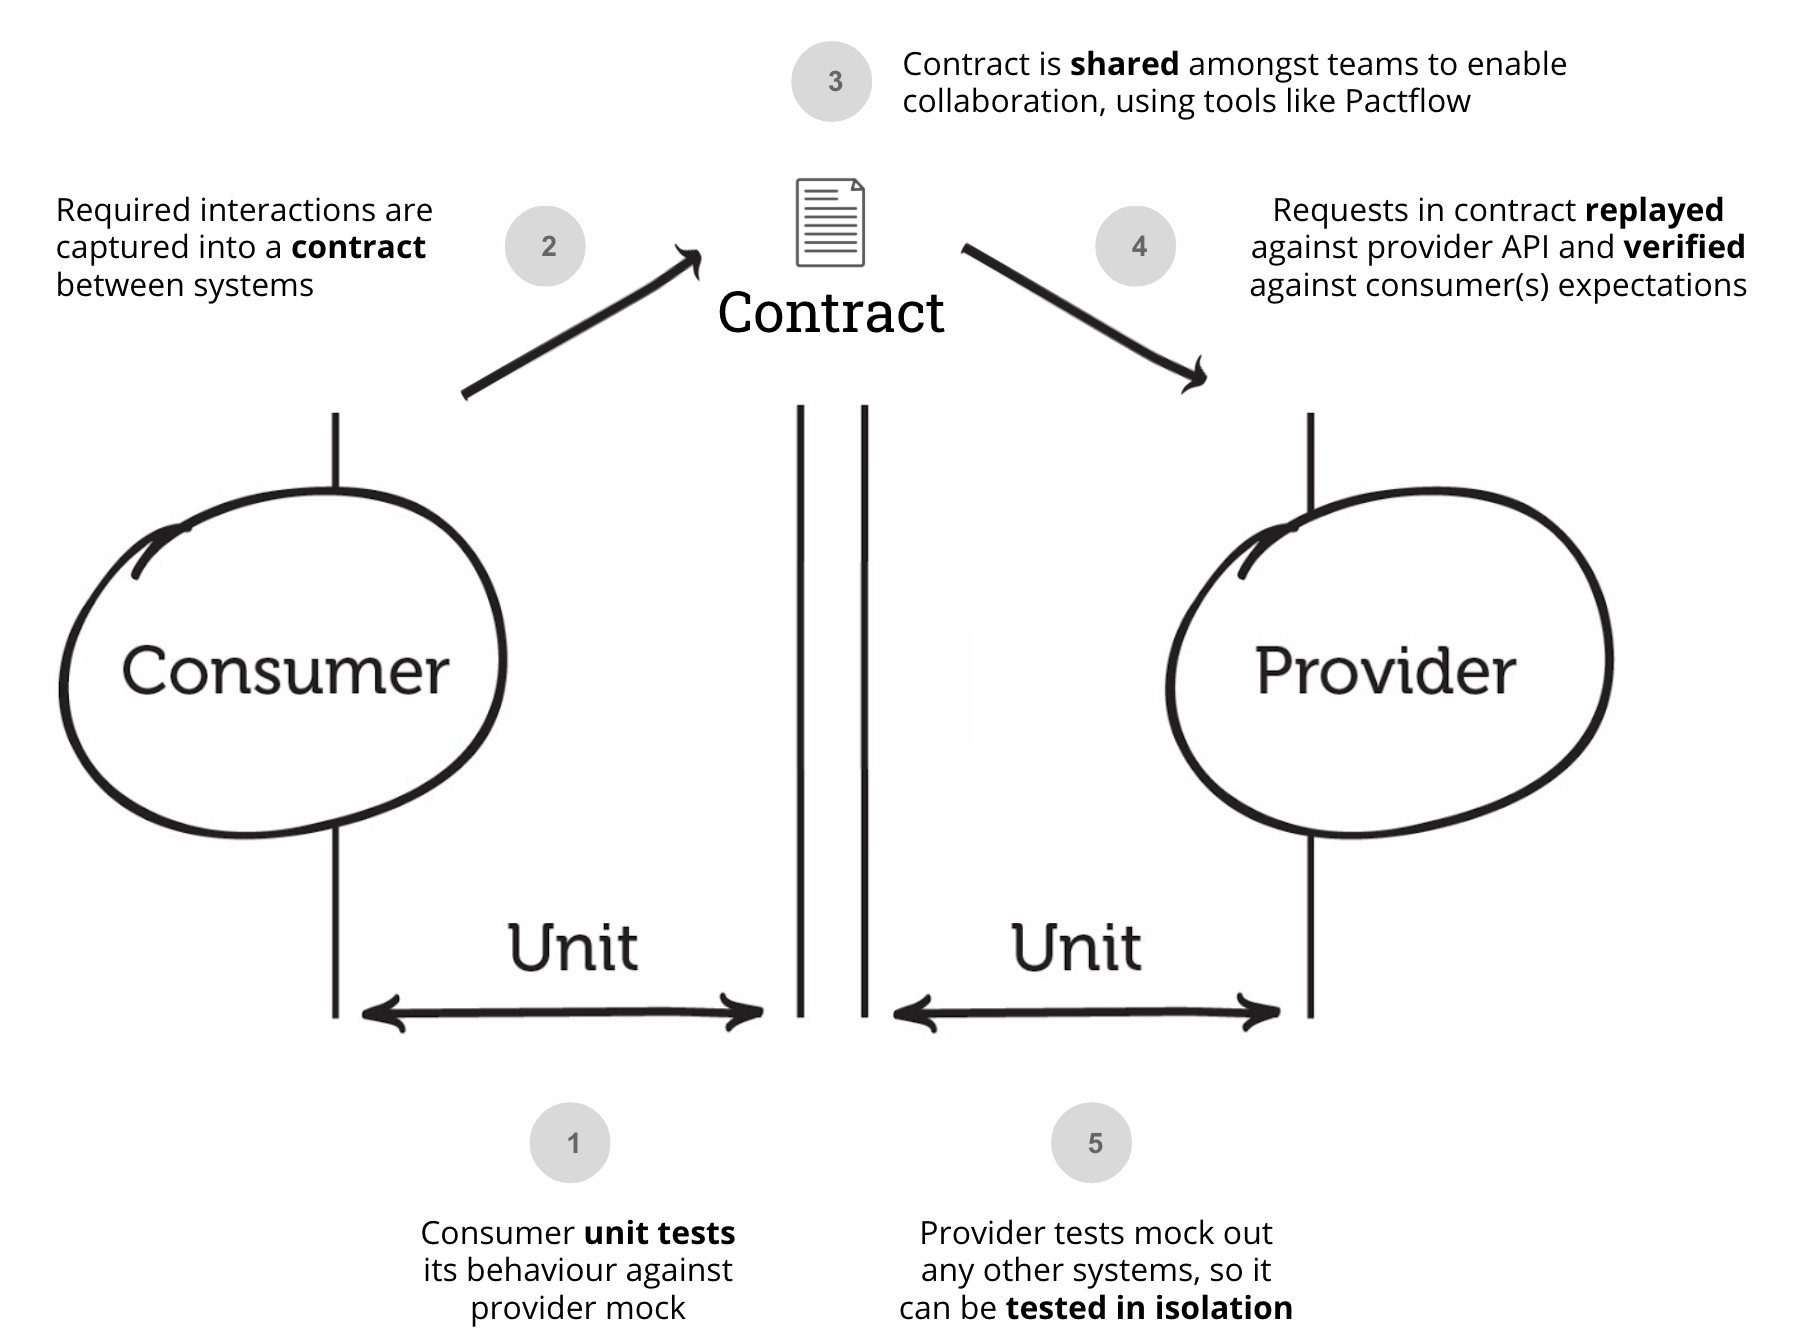
\includegraphics[width=.8\textwidth]{./assets/pact_overview}
    \end{center}
\end{frame}
